\documentclass[a4paper, 12pt]{article}
\usepackage[a4paper,top=1.5cm, bottom=1.5cm, left=1cm, right=1cm]{geometry}
\usepackage{cmap}					
\usepackage{mathtext} 				
\usepackage[T2A]{fontenc}			
\usepackage[utf8]{inputenc}			
\usepackage[english,russian]{babel}
\usepackage{multirow}
\usepackage{graphicx}
\graphicspath{ {./images/} }
\usepackage{wrapfig}
\usepackage{tabularx}
\usepackage{float}
\usepackage{ragged2e}
\usepackage{gensymb}
\usepackage{longtable}
\usepackage{hyperref}
\hypersetup{colorlinks=true,urlcolor=blue}
\usepackage[rgb]{xcolor}
\usepackage{amsmath,amsfonts,amssymb,amsthm,mathtools} 
\usepackage{icomma} 
\usepackage{euscript}
\usepackage{mathrsfs}
\usepackage{enumerate}
\usepackage{caption}
\usepackage{enumerate}
\usepackage{graphicx}
\usepackage{caption}
\usepackage{subcaption}

\DeclareMathOperator{\sgn}{\mathop{sgn}}
\newcommand*{\hm}[1]{#1\nobreak\discretionary{}
	{\hbox{$\mathsurround=0pt #1$}}{}}


\title{\textbf{Определение ускорения свободного падения при помощи оборотного маятника (1.4.2)}}
\author{Моргулёв Илья}
\date{Октябрь 28, 2023}

\begin{document}

\maketitle

\RaggedRight\textbf{Цель работы:} с помощью оборотного маятника измерить величину ускорения свободного падения. \newline
\textbf{В работе используются:} оборотный маятник с двумя подвесными призмами и двумя грузами (чечевицами); электронный счётчик времени и числа колебаний; подставка с остриём для определения центра масс маятника; закреплённая на стене консоль для подвешивания маятника; металлическике линейки, штангенциркуль длиной 1 метр.

\section{Введение}
\textbf{\textit{Теоретическая сводка:}}\newline
Для малых колебаний: \newline
\begin{equation}
\label{1}
T = 2 \pi \sqrt{\frac{J}{mgl}}
\end{equation}
Где $J$ - момент инерции маятника относительно оси качания, $l$ - расстояние от оси качания до центра масс маятника. \newline
Сравнивая эту формулу с уже известной всем из школьной программы $T = 2 \pi \sqrt{\frac{l}{g}}$. \newline
\begin{equation}
\label{2}
    l_{pr} = \frac{J}{ml}
\end{equation}
Где $l_{pr}$ - привеённая длина физического маятника. \newline
Смысл приведённой длины в том, что при длине математичсекого маятника, равной $l_{pr}$, его период колебаний совпадает с периодом колебаний физического маятника. \newline

\RaggedRight\textbf{Теорема Гюйгенса об оборотном маятнике} \newline
Пусть $\textit{O}_1$ — точка подвеса физического маятника, а $C$ — его центр масс. Отложим отрезок длиной $l_{pr}$ вдоль линии $\textit{O}_{1} \textit{C} $, и обозначим соответствующую точку как $\textit{O}_2$ — эту точку называют центром качания физического маятника. Заметим, что приведённая длина всегда больше расстояния до центра масс ($\textit{l}_{pr}$ > $\textit{l}$ ), поэтому точка $\textit{O}_2 $ лежит по другую сторону от центра масс. \newline

\begin{figure}[h!]
		\begin{center}
			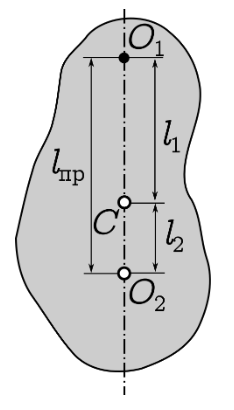
\includegraphics[width = 0.3\textwidth]{1.png}
			\caption{К теореме гюйгенса}
			\label{picture}
		\end{center}
	\end{figure}

Точки $\textit{O}_1$ и $\textit{O}_2$ обладают свойством взаимности: если перевернуть маятник и подвесить его за точку $\textit{O}_2$, то его период малых колебаний останется таким же, как и при подвешивании за точку $\textit{O}_1$ (теорема Гюйгенса). На этом свойстве — «оборотности» — и основан довольно точный метод определения ускорения свободного падения, применяемый в данной работе. Рисунок к работе теоремы гюйгенса приведён здесь: (\ref{picture}) \newpage
Докажем теорему Гюйгенса об оборотном маятнике. Пусть $\textit{O}_1$ и $\textit{O}_2$ — две точки подвеса физического маятника, лежащие на одной прямой с точкой $\textit{C}$ по разные стороны от неё. Тогда периоды колебаний маятника равны соответственно: \newline

\centering \begin{equation}
\label{3}
T_1 = 2 \pi \sqrt{\frac{J_1}{mg l_1}} ; \hspace{25} T_2 = 2 \pi \sqrt{\frac{J_2}{mg l_2}}
\end{equation}

По теореме Гюйгенса—Штейнера имеем:
\begin{equation}
\label{4}
    J_1 = J_c + ml_1^2 ; \hspace{25} J_2 = J_c + ml_2^2
\end{equation}
\RaggedRight где $J_c$ — момент инерции маятника относительно оси, проходящей через центр масс перпендикулярно плоскости качания.\newline
Пусть периоды колебаний одинаковы: $T_1 = T_2$ . Тогда одинаковы должны быть и приведённые длины:
\[
l_{pr} = \frac{J_1}{ml_1} = \frac{J_2}{ml_2}
\]

\RaggedRight С учётом (\ref{4}) имеем:
\begin{equation}
\label{5}
    l_{pr} = \frac{J_c}{ml_1} + l_1 = \frac{J_c}{ml_2} + l_2
\end{equation}
\RaggedRight откуда следует, что при $l_1 \neq l_2$ справедливо равенство:
\begin{equation}
\label{6}
    J_c = ml_1l_2
\end{equation}
\newpage
\RaggedRight Наконец, подставляя (\ref{6}) обратно в (\ref{5}), получим:
\begin{equation}
    \label{7}
    l_{pr} = l_1 + l_2
\end{equation}

\RaggedRightТаким образом, если периоды колебаний при подвешивании маятника в точках $\textit{O}_1$ и $\textit{O}_2$ равны, то расстояние между точками подвеса равно приведённой длине маятника. Нетрудно видеть, что и обратное утверждение также верно. 
Заметим также, что период колебаний маятника (\ref{3}), рассматриваемый как функция от $l_1$,
\[
T = 2\pi \sqrt{\frac{J_c + ml_1^2}{mgl_1}}
\]
имеет \textit{минимум} при $l_{1\textit{min}} = \sqrt{J_c/m}$. Из (\ref{6}) видно, что в этой точке $l_2 = l_1 = l_{pr}/2$, то есть центр масс находится посередине между сопряжёнными
точками $\textit{O}_1$ и $\textit{O}_2$ . График зависимости $T(l_1)$ схематично представлен на \ref{graf}
\begin{figure}[h!]
		\begin{center}
			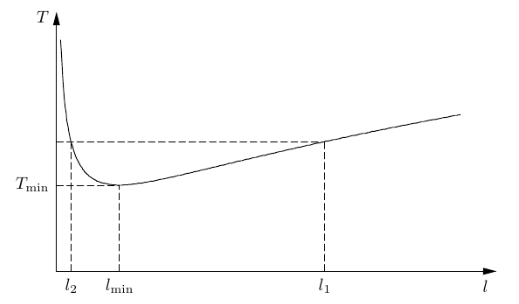
\includegraphics[width = 0.8\textwidth]{2.png}
			\caption{Зависимость периода колебаний от положения центра масс относительно оси качания}
			\label{graf}
		\end{center}
	\end{figure}
\newline

\RaggedRight\textbf{Измерение $g$}
Пусть $L \equiv \overline{O_1 O_2} = l_1 + l_2$ — расстояние между двумя «сопряжёнными»
точками подвеса физического маятника. Если соответствующие периоды
малых колебаний равны, $T_1 = T_2 = T$, то по теореме Гюйгенса $L = l_{pr}$. То-
гда из (\ref{1}) и (\ref{2}) находим ускорение свободного падения:
\begin{equation}
    \label{8}
    g_0 = (2\pi)^2 \frac{L}{T^2}
\end{equation}
\textit{Точного} совпадения $T_1 = T_2$ на опыте добиться, конечно, невозможно.
Поэтому получим формулу для определения ускорения свободного падения g, если измеренные периоды незначительно различаются: $T_1 = T$, $T_2 = T + \delta{T}$. Из системы (\ref{3}) и (\ref{4}) получаем:
\begin{equation}
    \label{9}
    g_0 = (2\pi)^2 \frac{l_1^2 - l_2^2}{T_1^2l_1 - T_2^2l_2}
\end{equation}
Отсюда следует, что $l_1/l_2$ желательно чтобы было не особенно близко к единице. На практике соблюдается следующее соотношение (желательно чтобы соблюдалось, в нашем эксперименте мы будем этого придерживаться):
\begin{equation}
    \label{10}
    l_1 > 2,5l_2
\end{equation}
\newpage
\textbf{Экспериментальная установка} \newline
Применяемые в работе маятники представляет собой стержни цилиндрического или прямоугольного сечения длиной $\approx$1 м и массой $\approx 1/1,5$ кг. Маятник подвешивается с помощью небольших треугольных призм (П1 и П2), острым основанием опирающихся на закреплённую на стене консоль. Ребро призмы задаёт ось качания маятника. На стержне закрепляются два дополнительных груза в форме «чечевицы» (Г1 и Г2). Для выполнения условия $L_1 > L_2$ внешнюю чечевицу Г2 следует крепить за призмой П2, а чечевицу Г1 (внутреннюю) — между призмами П1 и П2 (см. \ref{ustan}) \newline
\begin{figure}[h!]
		\begin{center}
			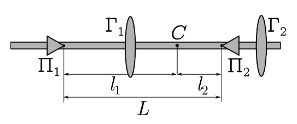
\includegraphics[width = 0.5\textwidth]{3.png}
			\caption{Маятник с двумя грузами}
			\label{ustan}
		\end{center}
	\end{figure}
Регистрация времени колебаний проводится с помощью электронных счётчиков. Расстояния между точками установки маятников на консоли до электронных счётчиков фиксировано. Это накладывает ограничения на расположение призм и грузов на стержне. Призмы крепятся \textit{симметрично} на равном расстоянии от концов стержней так, чтобы маятник при колебаниях пересекал фотоприёмники счётчика, не задевая оправу счётчика. \newline
Фиксированное положение призм однозначно задаёт приведённую длину оборотного маятника $l_{pr} = L$. Изменять в опыте можно только положения грузов на стрежне. Главная задача опыта — подобрать такое положение грузов, при котором периоды колебаний при перевороте маятника совпадали бы с достаточно высокой точностью, а для положения центра масс маятника выполнялось при этом условие (\ref{10}).\newline
\textbf{Предварительный расчёт положения грузов}\newline
Если первоначально расположить грузы на стержне произвольным образом, то для достижения равенства периодов колебаний потребуется исследовать зависимости периодов колебаний $T_1$ и $T_2$ при перемещении поочерёдно обоих грузов по штанге. При этом всякий раз необходимо при перестановке призм переворачивать тяжёлый маятник. Такая методика требует много времени и не всегда приводит к нужному результату.\newline
Существенно облегчить и ускорить поиск нужного положения грузов можно, если провести \textit{предварительные расчёты}. При этом для грубой оценки достаточно использовать максимально упрощённую модель, например, считать маятник \textit{тонким стержнем} с закреплёнными на нём точечными массами. После установки грузов согласно предварительным расчётам, их положение может быть уже уточнено экспериментально. \newline
Пусть призмы П1 и П2 задают сопряжённые точки подвеса, то есть период колебаний при перевороте маятника не изменяется. Тогда по теореме Гюйгенса расстояние между призмами $L$ — это приведённая длина маятника. Это условие может быть записано либо в форме (\ref{2}):
\begin{equation}
    \label{13}
    J_p = MLl_2,
\end{equation}
где $J_p$ — момент инерции маятника относительно призмы П2 , либо в форме (\ref{5}):
\begin{equation}
    \label{13'}
    J_c = Ml_1l_2
\end{equation}
где $J_c$ — момент инерции маятника относительно его \textit{центра масс}. Здесь $M$ — полная масса маятника.
Как $J_p$, так и $J_c$ являются функциями положений грузов $b_1$ и $b_2$ относительно соответствующих призм П1 и П2 (см. Рис. \ref{ustan2}). Задание длины $l_1$ (или $l_2$) определяет положение центра масс маятника. Это позволяет, во-первых, рассчитать правые части (\ref{13}) или (\ref{13'}), и, во-вторых, накладывает дополнительную связь на расстояния $b_1$ и $b_2$ (при известных массах всех элементов маятника). Тогда соотношения (\ref{13}) или (\ref{13'}) превращаются в уравнение с одной неизвестной, например, $b_2$. Корень этого уравнения можно приближённо найти графически, например, с помощью электронных таблиц. Дополнительные сведения о методике подбора положения грузов приведены в \ref{Приложение}.\newline
\textbf{Оценка погрешностей}
Оценим влияние погрешностей измерений на точность расчётов по формуле (\ref{9}). Пусть все периоды измерены с одинаковой погрешностью $\sigma_T $ , расстояние $L$ между точками подвеса с погрешностью $\sigma_L$ , расстояния $l_{1,2}$ до центра масс с погрешностью $\sigma_l$ Погрешность определения величины $g_0$
(по формуле (\ref{8})) равна: \newline
\begin{equation}
    \label{14}
    \frac{\sigma_{g_0}}{g_0} = \sqrt{(\frac{\sigma_L}{L})^2 + (\frac{\sigma_T}{T})^2 }.
\end{equation}
Это — основная погрешность опыта. Видно, что для её минимизации необходимо максимально точно измерить расстояние между точками повеса $L$ и период колебаний маятника $T$. \newline 
Проанализируем влияние поправки $g = g_0 + \Delta{g}$ : \newline
\[
\Delta{g} \approx \frac{2l_2}{l_1 - l_2}\cdot\frac{\Delta{T}}{T}g_0 .
\]
Общая формула для погрешности (\ref{9}) слишком громоздка, поэтому для наглядности анализа проведём вычисления приближённо. Достаточно учесть, что основной вклад в относительную погрешность $\Delta{g}$ вносят вели-
чины $\Delta{T}$ и $\Delta{l} = l_1 - l_2$, поскольку являются разностями двух близких ве-
личин. Поэтому \newline
\[
\frac{\Delta{g}}{g} \approx \frac{2(\frac{l_2}{l_1 - l_2}) \Delta{T}}{T} \sqrt{(\frac{\sigma_{\Delta{T}}}{\Delta{T}})^2 + (\frac{\sigma_{\Delta{l}}}{\Delta{l}})^2 }
\]
(здесь мы для воспользовались формулой погрешности разности, которая
даёт $\sigma_{\Delta{l}} = \sqrt{2}\sigma_{l}$ и $\sigma_{\Delta{T}} = \sqrt{2}\sigma_{T}$). Тогда для полной относительной погрешности получим \newline
\begin{equation}
    \label{15}
    \frac{\sigma_g}{g} \approx \sqrt{(\frac{\sigma_L}{L})^2 + 4(\frac{\sigma_T}{T})^2 + 8(\beta\frac{\sigma_T}{T})^2 8(\beta\frac{\Delta{T}}{T}\frac{\sigma_l}{\Delta{l}})^2} .
\end{equation}
Где $\beta$: \newline
\begin{equation*}
    \beta = \frac{l_2}{l_1 - l_2}
\end{equation*}
Из этого результата можно сделать следующие выводы. Во-первых, при достаточно хорошем совпадении периодов ($\Delta{T} \ll T$) погрешность измерения длин $l_1$ и $l_2$ по отдельности практически \textit{не влияет на погрешность конечного результата}, поскольку вклад последнего (4-го) слагаемого будет заведомо мал. И, во-вторых, итоговая погрешность \textit{неограниченно возрастает} при $l_1 \hookrightarrow l_2$ , т. е., когда центр масс маятника оказывается близок к геометрическому центру стержня. Проведём оценочные расчёты. Третье слагаемое в погрешности не превысит второе при $\sqrt{2}\beta < 1$, то есть \newline
\begin{figure}[h!]
		\begin{center}
			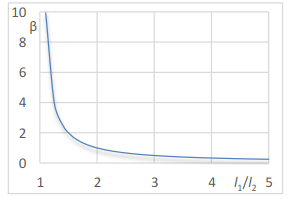
\includegraphics[width = 0.6\textwidth]{4.png}
			\caption{Зависимость коэффициента $\beta$ от положения центра масс}
			\label{grafic}
		\end{center}
	\end{figure}
\begin{equation*}
\label{uslovie}
    l_1 > (1 + \sqrt{2})l_2 \approx 2,4l_2
\end{equation*}
График зависимости относительной величины $\beta$ от $l_1/l_2$ приведён на Рис. \ref{grafic}.\newline
Оценим вклад последнего (4-го) слагаемого в (\ref{15}). Пусть погрешность измерения периода составляет $\frac{\sigma_T}{T} = \frac{0,01}{200} = 5\cdot10^-5$, а точность совпадения периодов при перевороте маятника равна $\Delta{T}/T \approx 10^-2 $ (1\%). Тогда для обеспечения заданной погрешности (4-е слагаемое не превышает остальные) длины $l_{1,2}$ достаточно измерять с относительной погрешностью $\sigma_l / l \approx 10^-2$ (1\%). Такая точность измерения положения центра масс вполне достижима на практике. Наконец, отсюда же видно, что при относительной погрешности определения положения центра масс в 1\% ($\sigma_l$ = 1 мм при $l \approx$ 10 см) нет необходимости добиваться совпадения периодов точнее, чем $\Delta{T}/T \approx$ 1\%

\section{Ход работы}
\begin{enumerate}
    \item Снимаем маятник с консоли и взвешиаем его. Снимаем грузы и призмы с маятника и взвешиваем все его элементы по отдельности (если элементы маятника являются несъёмными, соответствующие значения масс укaзаны на установке). \newline
\begin{tabular}{ll}\label{table:1}
Масса стержня                                  & 868,2 г                       \\
Масса призмы 1                                 & 78,4 г                        \\
Масса призмы 2                                 & 79,7 г                        \\
Масса груза 1                                  & 1483,7 г                      \\
Масса груза 2                                  & 1507,9 г                      \\
Масса маятника (вычисленная)                   & 4017,9 г                      \\
Масса маятника (измеренная)                    & 4017,9 г                      \\
Длина стержня                                  & 100 см                        \\
Расстояние между призмами                      & 59,6 см                       \\
Момент инерции стержня относительно призмы П2  & 0,176 кг*м\textasciicircum{}2 \\
Момент инерции маятника относительно призмы П2 & 0,416 кг*м\textasciicircum{}2 \\
L1/L2                                          & $\approx 2,7$                   \\
L1                                             & 44,2                          \\
L2                                             & 16,4                          \\
\end{tabular}
    \newline
    \vspace{10}
    Оценим погрешность измерения масс.\newline
    Данные измерений занесены в таблицу \ref{table:1}. Оценим погрешность измерений:
    \begin{center}
    $$\sigma_{sist} = 0,05 ; \hspace{25} \sigma_{rz} = 0,045 \\
    \sigma_m = \sqrt{\sigma_{sist}^2 + \sigma_{rz}^2} \approx 0,07 \\ $$
    \end{center}
    \item Закрепим подвесные призмы симметрично на стержне (положения призм указаны на установке). Убедимся, что ребра призм параллельны друг другу и «смотрят» в сторону центра маятника.    \newline
    \item С помощью большого штангенциркуля максимально точно измерим расстояние $L$ между призмами. В дальнейшем призмы должны оставаться закреплёнными на своих местах. \newline
    Оценим погрешность измерения длины. В таблице (\ref{table:1}) находятся данные измерений. \newline
    Погрешность измерения длины с помощью штангенциркуля $\sigma_L = 0,1$ мм, случайная погрешность у штангенциркуля отсутствует, следовательно общая погрешность равна систематической, равна 0,1 мм.\newline    
    \item Зададимся значением $l_1/l_2 = 2,4$ , удовлетворяющим условию (\ref{uslovie}), рассчитаем по методике, описанных в Приложении 1, положения грузов («чечевиц») на стержне.\newline
    Результаты измерений занесены в таблицу, закрепим грузы на соответствующих местах.    
    \item С помощью $\perp $-образной подставки определим положение центра масс маятника с грузами. Измерим расстояния $l_1$ и $l_2$ : от центра масс до острия призм П1 и П2 соответственно. Внесём данные в таблицу \ref{table:1} Убедимся, что условие \ref{uslovie}) выполнено: $l_1/l_2 \approx 2,695 \approx 2,7$ - условие \ref{uslovie} выполнено. Внесём результат в \ref{table:1}. \newline    
    \item Подвесим маятник на консоли на призме П2. Включаем электронный счётчик и убедимся в работоспособности системы (маятник при качании не касается элементов установки и не проскальзывает в подвесе, счётчик корректно считает количество колебаний и их время).\newline
    Маятник работает корректно, никаких задеваний не происходит, колебания считаются корректно.    
    \item Проведём измерение времени n = 20 колебаний 3–4 раза, вязкий раз отклоняя маятник на малый угол $\alpha \approx 5 \degree $. \newline
    Убедимся, что значения времён совпадают в пределах погрешности секундомера. \newline
    \begin{table}
        \centering
        \begin{tabular}{|c|c|c|c|}
        \hline
           $t_1$  & $t_2$ & $t_3$ & $t_4$ \\
           31,06  & 31,04 & 31,03 & 31,04\\
        \hline
        \end{tabular}
        \caption{Измерения времени для $n=20$}
        \label{tt}
    \end{table}
    В пределах погрешности значения совпадают. Погрешность секундомера\newline
    $\sigma_T = \sqrt{\sigma_{sl}^2+\sigma_{sist}^2} = \sqrt{0,027^2 + 0,005^2} \approx 0,027$    \newline
    Рассчитаем период колебаний $T_2$.\newline
    Для $n=20$ $T_2 = 31,04/20 \approx 1,55$ c.    
    \item Перевернём маятник, подвесив его на призму Π1 (при неизменном положении всех элементов на стержне). Проведём измерение периода $T_1$.\newline
    Для $n=20$ $T_1 = 31,15/20 \approx 1,56$ c.
    \item Сравним значения $T_1$ и $T_2$. Если различие не превышает $\Delta{T}/T \approx 1\%$, переходим к следующему пункту.\newline
    В противном случае, вернём маятник на призму Π 2, переместим груз Γ2 на небольшое расстояние (2–4 мм) и повторим измерения периодов по п. 7–8. При подборе положений грузов достаточно проводить каждый раз по одному измерению с n = 10 колебаний.\newline
    \[
    \frac{\Delta{T}}{T} \approx 6,4\cdot10^{-3}
    \]
    Это меньше 1\% , следовательно идём дальше.    
    \item Проведём окончательное измерение периодов $T_1$ и $T_2$ с максимальной точностью. Количество колебаний n примем \textit{100}. \newline
    Для $n=100$ 
    \begin{center}
    \begin{equation*}
        T_1=148,57/100 \approx 1,486\\
        T_2 \approx 1,486 \\
    \end{equation*} 
    \end{center}
           
    \item Снимем маятник с консоли.    
    \item Определим ускорение свободного падения g. Оценим погрешность конечного результата. Сравним результат с табличным.\newline
    По формуле \ref{9}:\newline
    \begin{equation*}
        g_0\approx 39,4\cdot\frac{0,168}{0,658} \approx 10,183
    \end{equation*}
    Тогда по формуле \ref{15}:
    \begin{equation*}
        \beta \approx 1,59\\
        \sigma_g \approx g_0\sqrt{ (\frac{0,0001}{59,6})^2 + 4(\frac{0,027}{1,486}^2) +8(\frac{1,59 \cdot0,027}{1,486})^2 +8(\frac{1,59\cdot0,04}{1,486} \cdot \frac{0,0001}{0,278})^2 } \approx 0,086 .
    \end{equation*}

    
\end{enumerate}

\section{Вывод}
В ходе данной раоты мы научились измерять погрешности при работе с цифровыми секундомерами и весами. Так же научились измерять силу тяжести с помощью оборотного маятника, познакомились с его устройством. Научилисьь автоматизировать процесс рассчёта некоторых формул с помощью таблиц. Разобрались с практическим применением теоремы Гюйгенса-Френейля. \newline
Так же рассчитали, что $g=(10,183\pm 0,083)$ кг*м/с$^2$.
\newpage


\section{Приложение}\label{Приложение}
Пусть $b_1$ — расстояние от груза Г1 до призмы П2, а $b_2$ — расстояние от груза Г2 до призмы П2 (см. Рис. \ref{ustan2}). Массы элементов маятника: стержня — $m_{st}$, подвесных призм — $m_{pr}$ и $m_{pr2}$, грузов — $m_1$ и $m_2$. \newline
\begin{figure}[h!]
		\begin{center}
			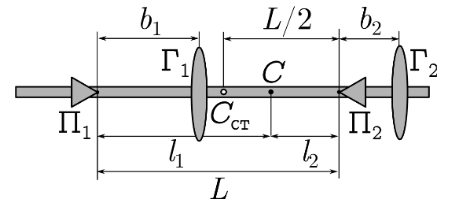
\includegraphics[width = 0.6\textwidth]{5.png}
			\caption{Расположение грузов и призм на маятнике. С — центр масс маятника, $C_{st}$ — центр масс стержня.}
			\label{ustan2}
		\end{center}
	\end{figure}
Будем считать положение центра масс маятника заданным. Тогда положения грузов $b_2$ и $b_1$ оказываются взаимно однозначно связаны соотношением: \newline
\begin{equation}
    \label{16}
    Ml_1 = m_{st}\frac{L}{2}+m_{pr2}L+m_1b_1+m_2(b_2+L) 
\end{equation}
где $M$ — полная масса маятника, $l_1$ —
расстояние от острия призмы П1 до центра масс маятника. Здесь мы считаем, что призмы расположены на стержне симметрично и центр масс стержня равноудалён на расстояние $L/2$ от призм. Все вычисления могут быть частично автоматизированы с помощью электронных таблиц.

    
\end{document}
